\documentclass[article, a4paper]{memoir}
\counterwithout{section}{chapter}
\usepackage[T1]{fontenc}
\usepackage[utf8]{inputenc}
\usepackage[a4paper]{geometry}
\geometry{verbose,tmargin=2.5cm,bmargin=2.5cm,lmargin=2.5cm,rmargin=2.5cm}
\usepackage{verbatim}
\usepackage{textcomp}
\usepackage{url}
\usepackage{amsmath}
\usepackage{graphicx}
\usepackage[spanish]{babel}
\usepackage[emulate=units]{siunitx}
\sisetup{per=fraction, fraction=nice, decimalsymbol=comma}
\usepackage{mathpazo}%Letra palatino con fuentes para matemáticas
\usepackage{esdiff}
\DeclareMathOperator{\di}{d\!}
\DeclareMathOperator{\ji}{\mathrm{j}}
\usepackage{steinmetz}

\author{Oscar Perpiñán Lamigueiro}
\date{}
\title{Repaso de trigonometría y números complejos}

\begin{document}

\maketitle

\section{Trigonometría}

\subsection{Ecuación Fundamental}

\begin{equation*}
  \sin^2(\alpha) + \cos^2(\alpha) = 1
\end{equation*}

\subsection{Cuadratura}

\begin{align*}
  \sin(\theta + \pi/2) &= \cos(\theta)\\
  \cos(\theta + \pi/2) &= -\sin(\theta)\\
  \sin(\theta - \pi/2) &= -\cos(\theta)\\
  \cos(\theta - \pi/2) &= \sin(\theta)
\end{align*}

\subsection{Suma y resta de ángulos}

\begin{align*}
  \cos(\alpha - \beta) &= \cos(\alpha) \cdot \cos(\beta) + \sin(\alpha) \cdot \sin(\beta)\\
  \cos(\alpha + \beta) &= \cos(\alpha) \cdot \cos(\beta) - \sin(\alpha) \cdot \sin(\beta)\\
  \sin(\alpha - \beta) &= \sin(\alpha) \cdot \cos(\beta) - \cos(\alpha) \cdot \sin(\beta)\\
  \sin(\alpha + \beta) &= \sin(\alpha) \cdot \cos(\beta) + \cos(\alpha) \cdot \sin(\beta)
\end{align*}

\subsection{Ángulo doble}

\begin{align*}
  \cos(2\alpha) &= 2 \cdot \cos^2(\alpha) - 1\\
  \cos(2\alpha) &= 1- 2 \cdot \sin^2(\alpha)
\end{align*}

\begin{equation*}
  \sin(2\alpha) = 2 \cdot \sin(\alpha) \cdot \cos(\alpha)
\end{equation*}

\subsection{Derivadas e Integrales}

\begin{align*}
  \diff{\sin(\omega t + \theta)}{t} = \omega \cdot \cos(\omega t + \theta)\\
  \diff{\cos(\omega t + \theta)}{t} = - \omega \cdot \sin(\omega t + \theta)
\end{align*}

\begin{align*}
  \int \sin(\omega t + \theta) \di t = -\frac{1}{\omega} \cdot \cos(\omega t + \theta) + k\\
  \int \cos(\omega t + \theta) \di t = \frac{1}{\omega} \cdot \sin(\omega t + \theta) + k
\end{align*}

Aprovechando las relaciones de cuadratura podemos comprobar que las derivadas adelantan $\pi/2$:

\begin{align*}
  \diff{\sin(\omega t + \theta)}{t} = \omega \cdot \sin(\omega t + \theta + \pi/2)\\
  \diff{\cos(\omega t + \theta)}{t} = \omega \cdot \cos(\omega t + \theta + \pi/2)
\end{align*}

Y las integrales retrasan $\pi/2$:
\begin{align*}
  \int \sin(\omega t + \theta) \di t = \frac{1}{\omega} \cdot \sin(\omega t + \theta - \pi/2) + k\\
  \int \cos(\omega t + \theta) \di t = \frac{1}{\omega} \cdot \cos(\omega t + \theta - \pi/2) + k
\end{align*}

\section{Números complejos}

\subsection{Definición}

\begin{minipage}{0.3\linewidth}
  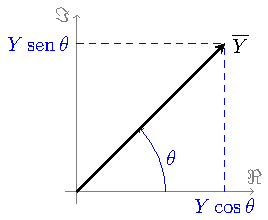
\includegraphics{../figs/fasor}  
\end{minipage}
\begin{minipage}{0.7\linewidth}
  Euler/Polar:
  \begin{align*}
    \overline{Y} &= Y\cdot e^{\ji\theta}\\
                     &= Y\phase{\theta}
  \end{align*}
  Binómica:
  \begin{align*}
    \overline{Y} &= Y \cdot \Big(\cos(\theta)+\ji\cdot\sin(\theta) \Big)\\
                 &= a_Y + \ji b_Y
  \end{align*}
\end{minipage}

\begin{align*}
  |Y| &= \sqrt{a^2_Y + b^2_Y} \\
      &=\sqrt{Y^2\cos^2(\theta) + Y^2\sin^2(\theta)}\\
      &= Y
\end{align*}

\subsection{Complejo unitario}

\begin{minipage}{0.3\linewidth}
  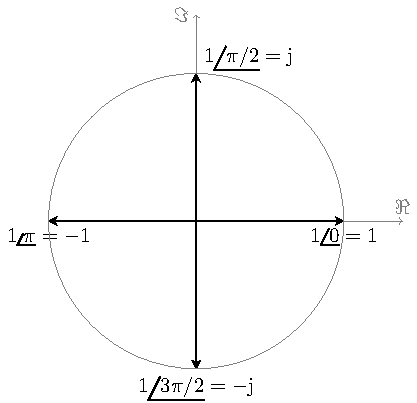
\includegraphics{../figs/circulo}
\end{minipage}
\begin{minipage}{0.7\linewidth}
  \begin{align*}
    1\phase{0} &= e^{\ji 0} = 1\\
    1\phase{\pi/2} &= e^{\ji \pi/2} = \ji\\
    1\phase{\pi} &= e^{\ji \pi} = -1\\
    1\phase{3\pi/2} &= e^{\ji 3\pi/2} = -\ji
  \end{align*}
\end{minipage}

\begin{minipage}{0.5\linewidth}
  \begin{align*}
    \ji^2 &= e^{\ji \pi/2} \cdot e^{\ji \pi/2}\\
          &= e^{\ji \pi}\\
          &= -1
  \end{align*}
\end{minipage}
\begin{minipage}{0.5\linewidth}
  \begin{align*}
    1/\ji &= 1/e^{\ji \pi/2} \\
          &= e^{-\ji \pi/2} \\
          &= e^{\ji 3\pi/2}\\
          &= -\ji
  \end{align*}
\end{minipage}

\subsection{Operaciones}

\begin{align*}
  \overline{Y} + \overline{Z} &= \Big(Y \cos(\theta_Y) + Z \cos(\theta_Z)\Big) + \ji \cdot \Big(Y \sin(\theta_Y) + Z \sin(\theta_Z)\Big)\\
  \overline{Y} - \overline{Z} &= \Big(Y \cos(\theta_Y) - Z \cos(\theta_Z)\Big) + \ji \cdot \Big(Y \sin(\theta_Y) - Z \sin(\theta_Z)\Big)
\end{align*}

\begin{align*}
  \overline{Y} \cdot \overline{Z} &= (Y \cdot Z )\cdot e^{\theta_Y + \theta_Z}\\
                                  &=(Y \cdot Z )\phase{\theta_Y + \theta_Z}\\
  \\
  \overline{Y}^2 &= Y^2\phase{2\theta_Y}\\
  \\
  \frac{\overline{Y}}{\overline{Z}} &= \frac{Y}{Z}\cdot e^{\theta_Y - \theta_Z}\\
                                  &= \frac{Y}{Z}\phase{\theta_Y - \theta_Z}
\end{align*}


\subsection{Conjugado}

\begin{align*}
  \overline{Y}^* &= Y\cdot e^{-\ji\theta}\\
                 &= Y\phase{-\theta}\\
                 &= Y \cdot \Big(\cos(\theta) - \ji\cdot\sin(\theta) \Big)\\
                 &= a_Y - \ji b_Y\\
  \\
  \overline{Y} \cdot \overline{Y}^* &= |Y|^2
\end{align*}


\end{document}